\lab{Algorithms}{Poisson's equation}{Poisson's equation}
\label{lab:finitedifference2}

% The basic idea behind finite difference methods is to replace a 
% differential operator, defined on some space of continuous functions, with a 
% difference operator defined on a finite vector space (i.e., a space of grid functions).
% 
% To do this, we replace derivative terms in the differential equation with 
% appropriate difference expressions. 
% 
% \begin{align*}
% 	u_{xx}(t,x) &\approx \frac{(u(t,x+h)- 2u(t,x) + u(t,x-h))}{h^2},\\
% 	u_x(t,x) & \approx \frac{u(t,x+h)-u(t,x-h)}{2h}.
% \end{align*}

Recall that the heat equation is given by $u_t = \nu u_{xx} + f(x,t,u)$. Suppose that we want to describe the flow of heat throughout a region $\Omega$. If the temperature on the boundary of $\Omega$ is fixed at $g$, and the $\Omega$ has an initial heat profile of $f$, then the flow of heat can be described by the boundary value problem 
\begin{align}
	\begin{split}
		& { } u_t = \nu \triangle u + f(x,t,u), \quad x \in \Omega, \quad t >0,\\
		& { }u(x,t) = h(x), \quad x \in \partial \Omega, \\
		& { }u(x,0) = g(x).
	\end{split}
\end{align}
When the source term $f$ does not depend on time, there is often a steady-state heat profile $u_{\infty}$ that is achieved as $t \to \infty$. This steady state $u_{\infty}$ is a solution of the boundary value problem 
\begin{align}
	\begin{split}
		& { }  \triangle u + f(x)/\nu = 0, \quad x \in \Omega,\\
		& { }u(x,t) = h(x), \quad x \in \partial \Omega.
	\end{split}
\end{align}
The partial differential equation $\triangle u = -f$ is commonly known as Poisson's equation. This equation is satisfied by the steady-state solutions of certain evolutionary processes. Poisson's equation is often used in electrostatics, image processing, and other areas. 

\section{Poisson's equation in one dimension}
Consider the boundary value problem defined by
\begin{align}
	\begin{split}
u'' &= f(x), \quad a \leq x \leq b,\\
	u(a) &= \alpha,\quad u(b) = \beta,
	\end{split}
\end{align}
where $f$ is continuous. 
The basic idea behind most numerical methods for differential equations is to 
approximate the exact solution $u(x)$ at some finite collection of points in the 
domain of the problem. Instead of analytically solving an infinite-dimensional
problem, we look for a simple finite collection of algebraic equations that approximate the original problem.

%Note that this equation can easily be solved by integrating twice 
%and using the boundary conditions to determine the constants of integration. 
Solving this boundary
value problem is equivalent to solving the equation $Du = f,$
where $D\frac{d^2}{dx^2}$ is a differential operator defined on the infinite-dimensional space 
of functions $u:[a,b] \to \mathbb{R}$ that are twice continuously differentiable and 
satisfy the boundary conditions $u(a) = \alpha$, $u(b) = \beta$. The finite difference method in general attempts to replace infinite-dimensional differential operators with finite difference operators. For example, recalling that $\frac{d^2}{dx^2}u(x) = \frac{1}{h^2}\left(u(x-h) -2u(x) + u(x+h)\right) + \mathcal{O}(h^2),$ we could  approximate $Du$ with the finite difference $\frac{1}{h^2}\left(u(x-h) -2u(x) + u(x+h)\right).$


We consider an approximate solution $\{u_i\}_{i=0}^N$ on an evenly spaced grid $a = x_0, x_1, \ldots, x_N = b$ with $h = x_{i+1}-x_i$ for each $i.$
We may discretize the boundary value problem as 
\begin{align*}
	\frac{1}{h^2} (u_{i+1}- 2u_i + u_{i-1})  &= f(x_i), \quad i = 1, \ldots, N-1,
\end{align*}
with the boundary conditions $u_0 = \alpha,$ $u_N = \beta.$ Note that this gives $N+1$ equations and $N+1$ unknowns. We can write this in matrix form as 
\[
\frac{1}{h^2} \begin{bmatrix}h^2 & 0 &0&\hdots &0 \\ 1 &-2 & 1 &\hdots &0\\ \vdots &  & \ddots & &\vdots \\
0 & \hdots & 1 & -2 & 1 \\ 0 & \hdots & & 0 & h^2
\end{bmatrix} \cdot \begin{bmatrix}y_0\\u_1\\ \vdots \\u_N\end{bmatrix} = \begin{bmatrix}f(x_0)\\f(x_1)\\ \vdots \\ f(x_N) \end{bmatrix}.
\]
We can further modify the system to obtain an $(N-1)\times (N-1)$ tridiagonal matrix on the left: 
\[
\frac{1}{h^2} \begin{bmatrix}-2 & 1 &0 & \hdots &0\\ 1 &-2 & 1 &\hdots &0\\ \vdots &  & \ddots & &\vdots \\ 0 & \hdots & 1 & -2 & 1 \\
0 & \hdots & 0 & 1 & -2 
\end{bmatrix} \cdot \begin{bmatrix}y_1\\y_2\\ \vdots \\y_{N-2}\\y_{N-1}\end{bmatrix} = \begin{bmatrix}f(x_1) -\alpha/h^2 \\f(x_2)\\ \vdots \\ f(x_{N-2})\\ f(x_{N-1})-\beta/h^2 \end{bmatrix}.
\]

The following code uses the finite difference method just described to solve the boundary value problem
\begin{align*}
u'' &= -3 \sin{x}, \quad 0 \leq x \leq 2,\\
	u(0) &= -2,\quad u(2) = 1.
\end{align*}
Note the use of matrix functions from \li{scipy.sparse}. %Several variations of this matrix will be built throughout this lab. 

\begin{lstlisting}
from __future__ import division
import numpy as np
from scipy.sparse import spdiags
from scipy.sparse.linalg import spsolve

def bvp(func,a=0.,b=2.,alpha=-1.,beta=3.,N = 5):
	h = (b-a)/N 				# The length of each subinterval
	
	# Initialize and define the vector F on the right
	F = np.empty(N-1.)			
	F[0] = func(a+1.*h)-alpha*h**(-2.)
	F[N-2] = func(a+(N-1)*h)-beta*h**(-2.)
	for j in xrange(1,N-2): 
		F[j] = func(a + (j+1)*h)
	
	# Here we define the arrays that will go on the diagonals of A
	D0, D1 = -2.*np.ones((1,N-1)), np.ones((1,N-1))  
	# Next we concatenate the arrays, and specify on which diagonals they will be placed
	diags = np.array([0,-1,1])
	data = np.concatenate((D0,D1,D1),axis=0) 
	A=h**(-2.)*spdiags(data,diags,N-1,N-1).asformat('csr')
	
	# We create and return the numerical approximation
	U = spsolve(A,F)
	U = np.concatenate( ( np.array([alpha]), U, np.array([beta]) ) )
	return np.linspace(a,b,N+1), U

x, y = bvp(lambda x:(-3.*np.sin(x)), a=0., b=2., alpha=-2., beta=1, N=30)
\end{lstlisting}

% How do we know if a numerical approximation is reasonable?  One way to determine this is to compute solutions for various step sizes $h$ and see if the solutions are converging to something.  To be more specific, suppose our finite difference method is $\mathcal{O}(h^p)$ accurate.  This means that the error $E(h) \approx Ch^p$ for some constant $C$ as $h \to 0$ (i.e., for $h>0$ small enough).
% 
% So compute the approximation $y_k$ for each stepsize $h_k$, $h_1 > h_2> \ldots>h_m.$  We will think of $y_m$ as the true solution.  Then the error of the approximation for 
% stepsize $h_k, k < m,$ is 
% \begin{align*}
% 	E(h_k) &= \max( \abs{ y_k - y_m}) \approx C h_k^p ,\\
% 	\log(E(h_k)) &= \log(C) + p \log(h_k).
% \end{align*}
% Thus on a log-log plot of $E(h)$ vs. $h,$ these values should be on a straight line with slope $p$ when $h$ is small enough to start getting convergence. 

% The following code generates the log-log plot in \ref{figure1}, and demonstrates second-order convergence for this finite difference approximation. 
% \begin{lstlisting}
% import matplotlib.pyplot as plt
% a, b = 0., 1.
% num_approx = 10 # Number of Approximations
% N = np.array([5*2**j for j in range(num_approx)])
% h, max_error = (b-a)/N[:-1], np.ones(num_approx-1)
% 
% mesh_best, num_sol_best = bvp(lambda x:-3.*np.sin(x), a, b, alpha=-2., beta=1, N=N[-1])
% for j in range(len(N)-1): 
%     mesh, num_sol = bvp(lambda x:-3.*np.sin(x), a, b, alpha=-2., beta=1, N=N[j])
%     max_error[j] = np.max(np.abs( num_sol- num_sol_best[::2**(num_approx-j-1)] ) )
% plt.loglog(h,max_error,'.-r',label="$E(h)$")
% plt.loglog(h,h**(2.),'-k',label="$h^{\, 2}$")
% plt.xlabel("$h$")
% plt.legend(loc='best')
% plt.show()
% print "The order of the finite difference approximation is about ", ( (np.log(max_error[0]) - 
%     np.log(max_error[-1]) )/( np.log(h[0]) - np.log(h[-1]) ) ), "."
% \end{lstlisting}

\begin{figure}[ht]
\centering
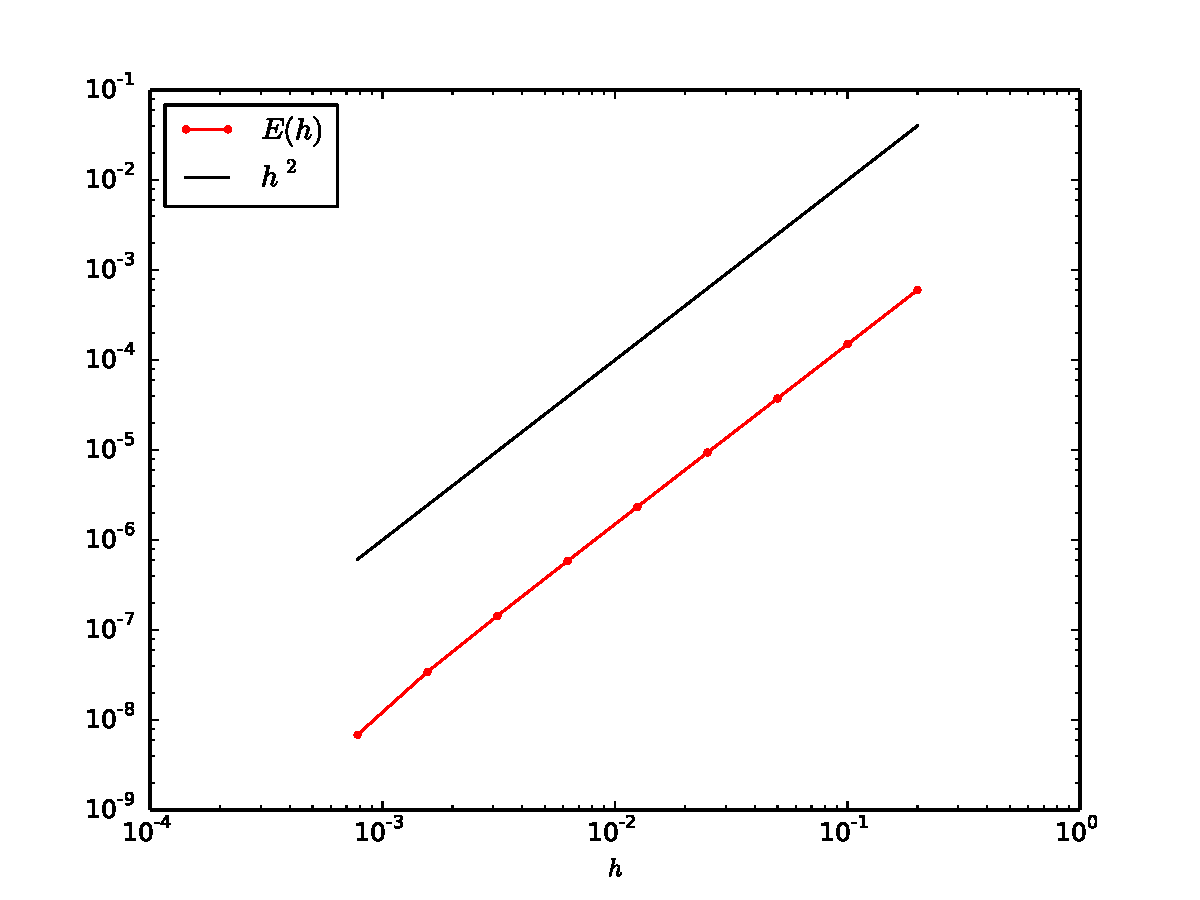
\includegraphics[width=12cm]{example_convergence.pdf}
\caption{TODO}
\label{figure1}
\end{figure}


\begin{problem}
Extend the given finite difference code to the case of a general second order linear boundary value problem with Dirichlet conditions:
\begin{align*}
	&{ } a_1(x)y'' +a_2(x)y'+ a_3(x) y = f(x), \quad x \in (0,1),\\
	&{ } y(0) = \alpha, \quad y(1) = \beta.
\end{align*}
Use your code to solve the singularly perturbed boundary value problem
\begin{align*}
	&{ } \epsilon y''(x)-y'= f(x), \quad x \in (0,1), \\
	&{ } y(0) = 1, \quad y(1) = 3,
\end{align*}
with $\epsilon = 1/10$. How many subintervals are needed to obtain 4 digits of accuracy? 

% If $\alpha = 1,$  $\beta = 3,$ and $f(x) = -1$, there is an exact solution: 
% \[y(x) = \alpha + x+ (\beta - \alpha -1)\frac{e^{x/\epsilon -1}}{e^{1/\epsilon -1}}
% .\]
\end{problem}

\begin{figure}[ht]
\centering
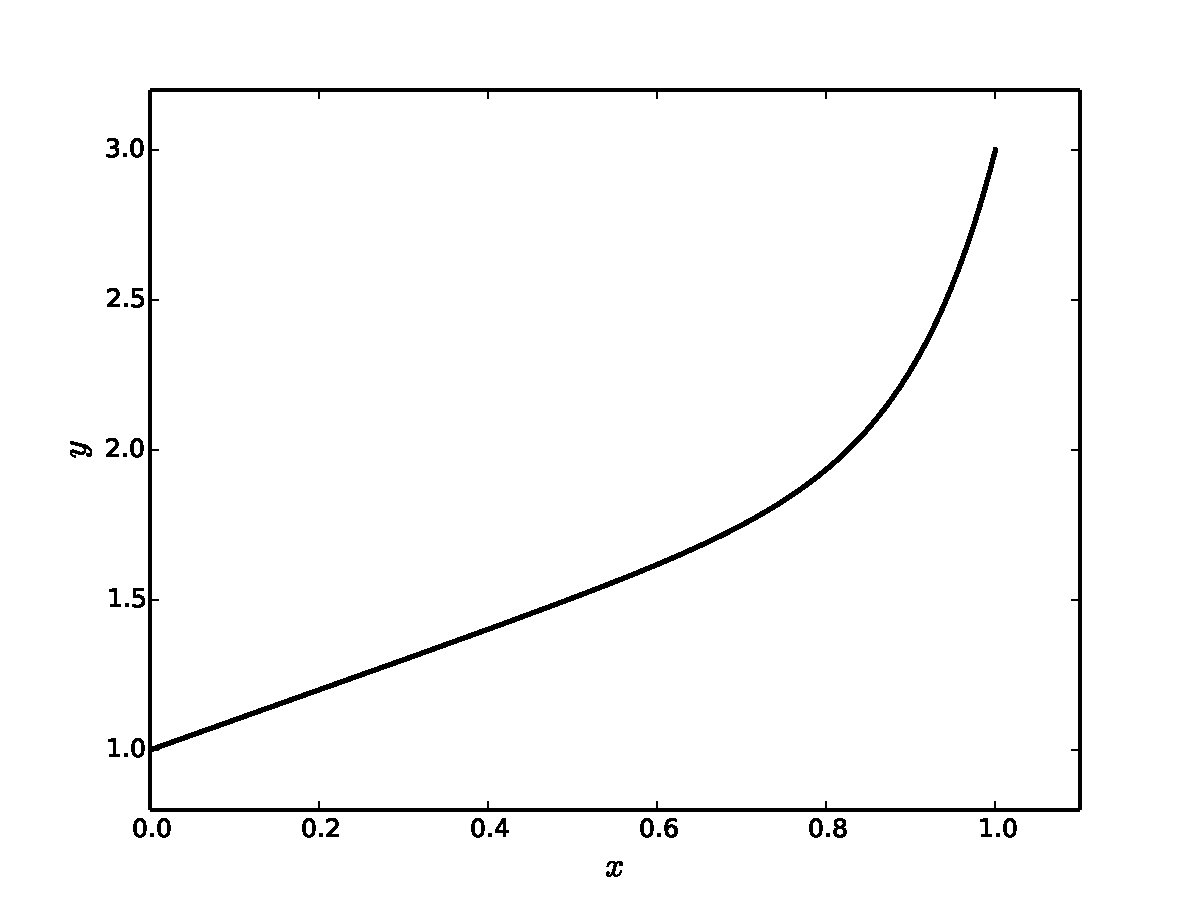
\includegraphics[width=12cm]{figure2.pdf}
\caption{TODO}
\label{figure2}
\end{figure}



\section{Poisson's equation in two dimensions}

% Consider Poisson's equation together with Dirichlet boundary conditions on a square domain:
% \begin{align*}
% 	u_{xx} + u_{yy} &= f,\quad x \text{ in } [0,1]\times[0,1] \subset \mathbb{R}^2,\\
% 	u &= g, \quad x \text{ on } \partial \left( [0,1]\times[0,1]\right).
% \end{align*}
% We will use the finite difference approximation
% \begin{align*}
% u_{xx}(x,y) + u_{yy}(x,y) &= \frac{u(x+h,y) - 2u(x,y)+ u(x-h,y)}{h^2} \\
% & \qquad{}+ 
% \frac{u(x,y+h) - 2u(x,y)+ u(x,y-h)}{h^2} + \mathcal{O}(h^2).
% \end{align*}
% Define the difference operator $\nabla^2_h$ by 
% \[
% \nabla^2_h U_{ij} = \frac{1}{h^2}(U_{i-1,\,j} + U_{i+1,\,j} + U_{i,\,j-1} + U_{i,\,j+1}-4U_{i,\,j}).
% \]
% Then the set of equations  $\nabla^2_h U_{ij} = f_{ij}$, $i,j = 1,\ldots,m$ can be written in matrix form as
% $$AU + q  = f$$
% Here $A$ is the block tridiagonal matrix 
% \[
% \frac{1}{h^2} \begin{bmatrix}T & I & &  &\\ I &T & I & &\\  &\ddots  & \ddots & \ddots & \\  &  & I & T & I \\
%  &  &  & I & T
% \end{bmatrix}
% \]
% where $I$ is the $m\times m$ identity matrix, and $T$ is the tridiagonal matrix
% \[
%  \begin{bmatrix}-4 & 1 & &  &\\ 1 &-4 & 1 & &\\  &\ddots  & \ddots & \ddots & \\  &  & 1 & -4 & 1 \\
%  &  &  & 1 & -4
% \end{bmatrix}.
% \]

% The vector $U$ is given by 
% \[
% U = \begin{bmatrix} U^1 \\ U^2 \\ \\ U^m \end{bmatrix} \text{ where } U^j = 
% \begin{bmatrix} U_{1,\,j} \\ U_{2,\,j} \\ \\ U_{m,\,j} \end{bmatrix} \text{ for each } j, 1\leq j \leq m.
% \]
% So $U^j$ represents the $j$th row of interior points in our grid, where $y_j = jh.$
% 
% 
% The vector $q$ is given by $u = [q^1 \ldots q^m]^T$, where 
% \[
% q^j = \frac{1}{h^2}
% \begin{bmatrix} g_{0,\,j} \\ 0 \\ \vdots \\0\\ g_{m+1,\,j} \end{bmatrix} , \,\,\, 2 \leq j \leq m-1,
% \]
% and 
% \[
% q^1 = \frac{1}{h^2}\begin{bmatrix} g_{1,0} + g_{0,1} \\ g_{2,0} \\ \vdots \\ g_{m-1,0}\\ g_{m,0} + g_{m+1,1}\end{bmatrix}, \quad q^m = \frac{1}{h^2}\begin{bmatrix} g_{1,m+1} + g_{0,m}\\ g_{2,m+1} \\ \vdots \\ g_{m-1,m+1}\\ g_{m,m+1} + g_{m+1,m}\end{bmatrix}.
% \]

\begin{problem}
	Find the solution $u$ of the 2D Laplace equation $\Delta u = 0$ on the unit 
	square $[0,1]\times [0,1] \subset \mathbb{R}^2,$ subject to the (Dirichlet) condition that 
	$u(x,y) = x^3$ on the boundary. 
	% 
	% Graph your solution, and demonstrate convergence of the numerical approximation by 
	% creating a log-log plotof the error $E(h).$
\end{problem}

\begin{problem}
	Find the solution $u$ of the 2D Poisson equation with the given Dirichlet boundary conditions:
	\begin{align*}
		\Delta u &= -\pi^2 \sin(\pi x)\sin(\pi y), \quad (x,y) \in [0,1]\times [0,1], \\
		u(x,0) &= 1-x, \\
		u(x,1) &= 1-2x, \\
		u(0,y) &= 1, \\
		u(1,y) &= -y. 
	\end{align*}
	
	Graph your solution, and demonstrate convergence of the numerical approximation by 
	creating a log-log plot of the error $E(h).$
\end{problem}

% The matrix $A$ is sparse, and so we can use several functions from the package \texttt{scipy.sparse.linalg}. In particular, we use the functions \texttt{spdiags} and \texttt{spsolve}.
% 
% 
% 
% 
% \begin{verbatim}
% D1,D2,D3 = -4*np.ones((1,m**2)), np.ones((1,m**2)), np.ones((1,m**2)) 
% Dm = np.ones((1,m**2))
% for j in range(0,D2.shape[1]):
%     if (j%m)==m-1:
%         D2[0,j]=0
%         if (j%m)==0:
%             D3[0,j]=a0
% diags = np.array([0,-1,1,-m,m])
% data = np.concatenate((D1,D2,D3,Dm,Dm),axis=0)
% 
% A = 1./h**2.*spdiags(data, diags, m**2,m**2).asformat('csr') 
% \end{verbatim}
% 
% \subsection{2D Heat Equation}
% Recall that the collection of finite difference equations
% \[
% \nabla^2_h U_{ij} = 0, \quad 1 \leq i,j\leq m,
% \]
% can be written in matrix form as
% $$AU + q  = 0$$
% 
% 
% The Crank-Nicolson method for the 2D heat equation is given by 
% $$U_{i,\,j}^{n+1}- U_{i,\,j}^{n} = \frac{\Delta t}{2}(\nabla_h^2 U_{i,\,j}^{n} + \nabla_h^2 U_{i,\,j}^{n+1}) \text{ for each } 1 \leq i,j \leq m, $$
% is a second order accurate in both space and time. Basically we're using a midpoint scheme in time, 
% and a trapezoidal scheme in space. The resulting method is implicit, and can be written in matrix form as 
% \begin{align*}
% 	IU^{n+1} &= IU^n + \frac{\Delta t}{2}(AU^n + q + AU^{n+1} + q),\\
% 	(I - \frac{\Delta t}{2}A)U^{n+1}&= (I + \frac{\Delta t}{2}A)U^n + \Delta t q.	
% \end{align*}
% 
% 
% 
% TODO: What size must the time step be to ensure stability? 
% 
% We will need to take many time steps, where many equations must be solved with the matrix $(I - \frac{\Delta t}{2}A)$. The function \texttt{factorized} from \texttt{scipy.sparse.linalg} computes the LU decomposition of the matrix. This decomposition reduces the time required for solving consecutive time steps. 
% 
